\documentclass[conference]{IEEEtran}
\usepackage{booktabs}
\usepackage{graphicx}
\usepackage{amsmath}
\usepackage{url}
\usepackage{xcolor}
\usepackage{multirow}
\usepackage{microtype}
\usepackage{algorithm}
\usepackage{algpseudocode}

\title{High Accuracy, Low Assurance: Auditing Outcome-Proxy Sensitivity, Geographic Transportability, and Uncertainty in Student-Depression Prediction}

% Replace only after the venue's anonymity policy permits author disclosure.
\author{\IEEEauthorblockN{Anonymous Author(s)}
\IEEEauthorblockA{Anonymous Institution\\Under double-blind review}}

\begin{document}
\maketitle

\begin{abstract}
Machine-learning studies of student depression often emphasize discrimination while giving less attention to outcome definition, construct overlap, transportability, and uncertainty. We audit a public survey dataset containing 4,464 student records from Bangladesh and a binary self-reported depression indicator (26.9\% positive). The feature \emph{Health condition} exhibited near-deterministic overlap with the outcome: all 634 students reporting ``Critical'' health were positive, whereas all 1,162 reporting ``Good'' health were negative. We therefore compared a full-predictor setting with a prespecified proxy-free sensitivity setting that excluded this feature. Five model families were evaluated using nested 5$\times$3-fold cross-validation, bootstrap confidence intervals, leave-one-home-division-out validation, subgroup error audits, and split-conformal prediction. In nested cross-validation, the selected full Random Forest achieved AUPRC 0.998 (95\% CI 0.997--0.999) and AUROC 0.999 (0.999--1.000). Removing health condition reduced the selected HistGradientBoosting model to AUPRC 0.520 (0.491--0.551) and AUROC 0.751 (0.735--0.766). Under division-held-out evaluation, proxy-free performance fell further to AUPRC 0.452 and AUROC 0.691, with a false-negative-rate range of 0.284 across divisions. Across five 90\% split-conformal runs, mean marginal coverage was 0.903, but only 60.9\% of test cases received singleton sets. These findings show that near-perfect internal performance can principally reflect an outcome-proximal variable and should not be interpreted as evidence of deployable screening. The contribution is a reproducible stress-test protocol for outcome-proxy dependence, subgroup reliability, transportability, and abstention in high-stakes tabular prediction.
\end{abstract}

\begin{IEEEkeywords}
student depression, outcome proxy, construct overlap, nested cross-validation, fairness audit, conformal prediction, transportability
\end{IEEEkeywords}

\section{Introduction}
Depression among students is an important public-health and educational concern. Predictive models built from demographic, academic, social, and lifestyle variables are increasingly proposed to support earlier identification of students who may need assessment. Recent studies combine ensemble learning with SHAP explanations, decision-curve analysis, fairness evaluation, or counterfactual explanations \cite{chang2026interpretable,isiwu2026multilevel}. These additions improve transparency, yet a more basic question precedes model explanation: \emph{what signal is the model learning?}

An apparently excellent model may rely on a predictor that is contemporaneous with, semantically overlaps, or partially encodes the outcome. Such a feature is not necessarily erroneous; it can be useful in a clearly defined concurrent classification task. However, its presence can make performance unsuitable evidence for early, non-clinical screening. This concern is especially consequential when the public data card does not document the exact outcome question, temporal ordering, or validated instrument.

Current prediction-model guidance distinguishes model development from unbiased performance evaluation and emphasizes outcome definition, predictor measurement, calibration, external validation, and fairness \cite{collins2024tripod,moons2025probast}. We operationalize these principles as an empirical audit of a public student-depression dataset. Rather than proposing a new classifier, we ask how conclusions change when the strongest potential outcome proxy is removed and when home-division groups are held out.

Our contributions are fourfold:
\begin{enumerate}
    \item a transparent audit that identifies near-deterministic conditional outcome rates for the self-reported health-condition variable;
    \item leakage-safe nested comparisons of full and proxy-free feature settings across five model families;
    \item geographic-group transportability and subgroup error audits covering gender, family background, and home division; and
    \item uncertainty-aware evaluation through repeated split-conformal prediction and selective classification.
\end{enumerate}

We deliberately do not call the outcome a clinical diagnosis. The available documentation describes only a binary depression indicator and does not identify PHQ-9, CES-D, clinician assessment, or another validated reference standard \cite{haque2026dataset}.

\subsection{Research Questions}
The study is organized around four questions. \textbf{RQ1:} How much of the apparent predictive performance depends on the potential outcome proxy? \textbf{RQ2:} Do relative conclusions persist when an entire home-division group is unseen during development? \textbf{RQ3:} Are threshold errors and probability error stable across demographic, socioeconomic, and geographic subgroups? \textbf{RQ4:} How often can a proxy-free model issue an informative singleton prediction while attaining nominal conformal coverage? These questions separate discrimination from construct validity, transportability, group reliability, and uncertainty.

\begin{figure*}[t]
\centering
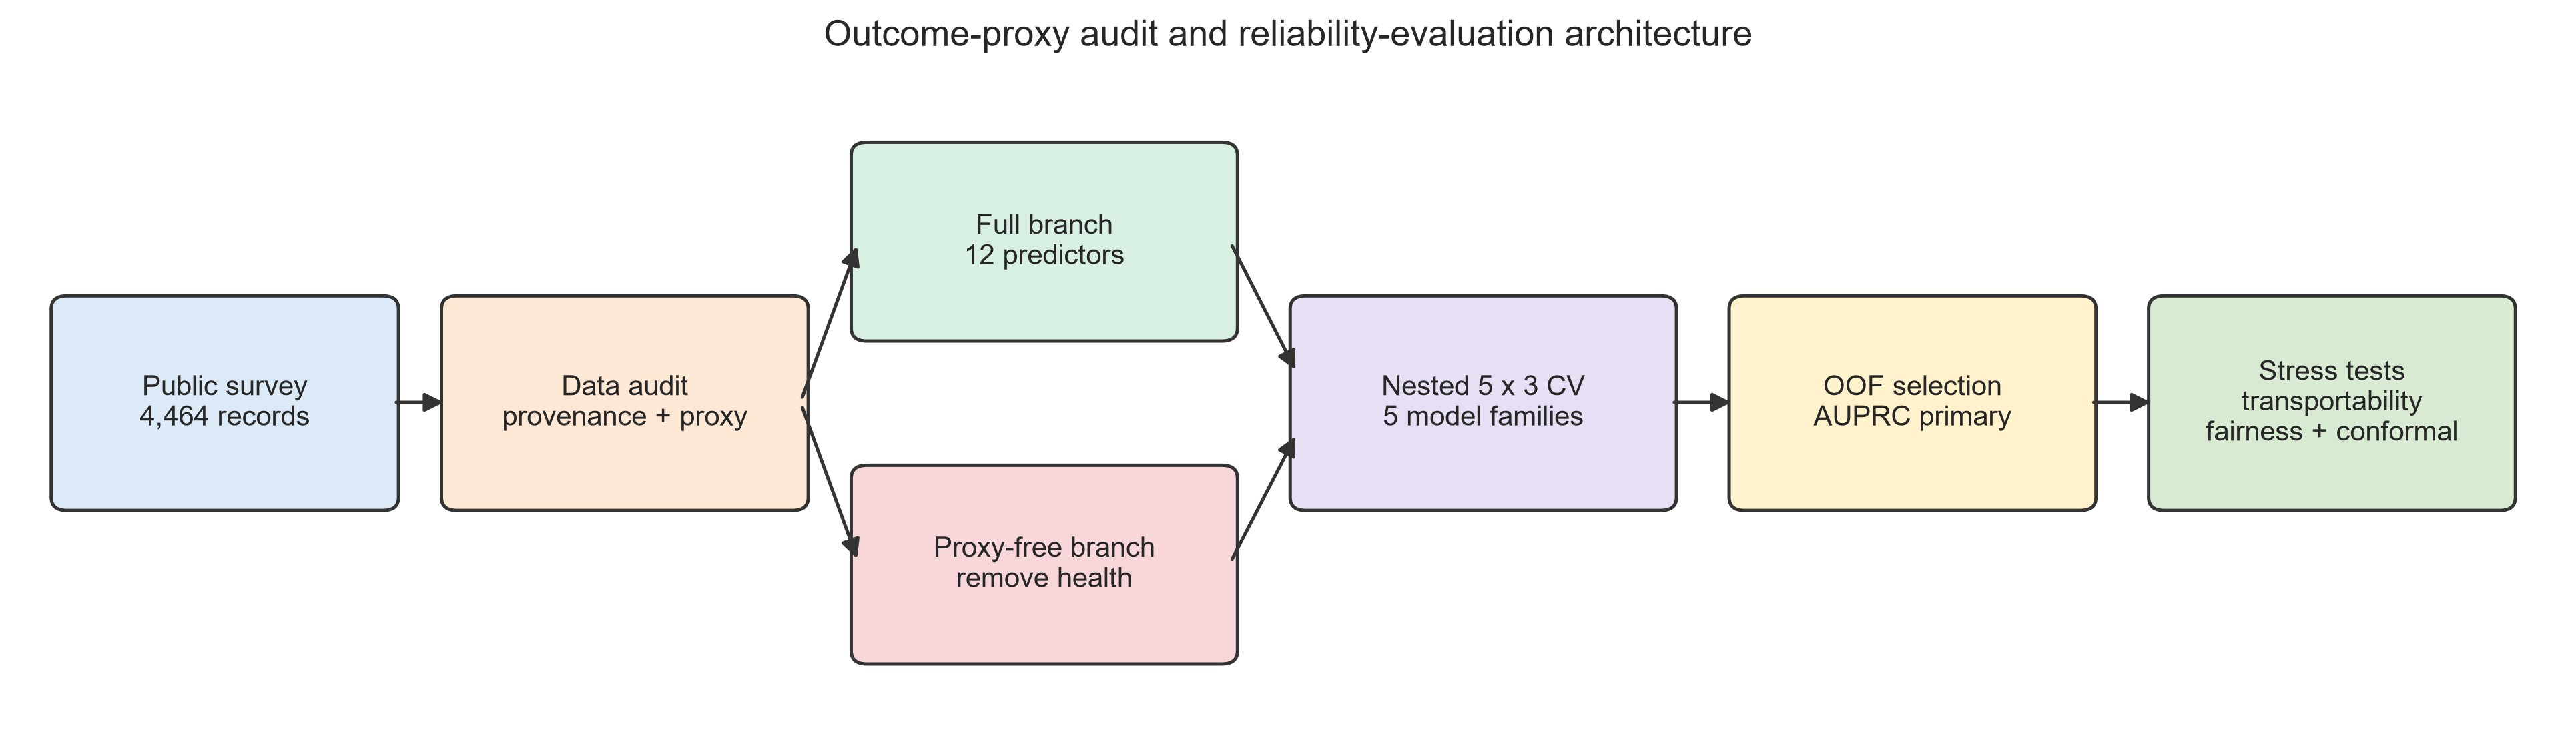
\includegraphics[width=0.96\textwidth]{../artifacts/figures/figure_7_study_architecture.png}
\caption{End-to-end architecture. Data auditing precedes the full and proxy-free branches. Hyperparameter selection occurs only within inner folds; outer-fold predictions drive model selection and reliability stress tests.}
\label{fig:architecture}
\end{figure*}

\section{Related Work}
\subsection{Student-depression prediction}
Recent student-depression research has moved beyond accuracy-only comparisons. Chang \cite{chang2026interpretable} combined XGBoost and SHAP with calibration and decision-curve analysis, reporting that a sensitivity model excluding suicidal ideation retained useful discrimination. Isiwu et al. \cite{isiwu2026multilevel} studied global, subgroup, and individual explanations. Such sensitivity analyses motivate asking whether other highly proximal predictors dominate apparent performance.

\subsection{Fairness and uncertainty}
Depression-prediction models can differ materially across demographic and socioeconomic groups. Dang et al. \cite{dang2024fairness} found no universally best accuracy--fairness combination across four populations and emphasized subgroup monitoring. Cheong et al. \cite{cheong2025ufair} connected uncertainty, gender-based reweighting, and fairness in multimodal depression detection, while also reporting negative transfer. Our study does not propose a fairness intervention. Instead, it reports false-negative, false-positive, and calibration gaps so that aggregate performance does not conceal subgroup behavior.

Conformal prediction converts probabilistic scores into prediction sets with finite-sample marginal coverage under exchangeability \cite{vovk2005algorithmic,angelopoulos2023gentle}. It is attractive for high-stakes screening because a model can return a non-singleton set rather than force a binary answer. Coverage is nevertheless marginal, not automatically subgroup-conditional, and can fail under distribution shift.

\section{Data, Outcome, and Ethics}
\subsection{Dataset}
We used Version 2 of the \emph{Student Depression Detection Dataset}, distributed under CC BY 4.0 with DOI \texttt{10.17632/xn9cb5zpgg.2} and mirrored publicly on Kaggle \cite{haque2026dataset}. The data card describes Google Forms collection and 4,464 student records. The complete SHA-256 of the analyzed CSV is reported in the reproducibility repository.

The 12 candidate predictors cover gender, age, family background, relationship status, marital status, living style, current semester, CGPA, friend circle, health condition, monthly cost excluding study, and home division. The binary outcome contains 1,201 positive (26.9\%) and 3,263 negative records. There were no missing cells or exact duplicate rows.

\subsection{Outcome boundary}
The public metadata does not state the outcome question, recall window, threshold, or diagnostic instrument. We consequently use the term \emph{self-reported depression indicator}. Results cannot establish major depressive disorder, severity, onset, prognosis, or need for treatment. The study uses de-identified public secondary data and makes no individual decisions.

\subsection{Potential outcome proxy}
Table~\ref{tab:health} shows that health condition is nearly deterministically associated with the outcome. Because the questionnaire wording and temporal relationship are unavailable, we do not assert that this is proven leakage. We treat it as a potential outcome proxy or construct-overlap variable and prespecify a sensitivity analysis excluding it.

\begin{table}[t]
\centering
\caption{Outcome rate by self-reported health condition.}
\label{tab:health}
\begin{tabular}{lrrr}
\toprule
Health condition & $n$ & Positive & Rate \\
\midrule
Critical & 634 & 634 & 1.000 \\
Abnormal & 881 & 484 & 0.549 \\
Normal & 1,787 & 83 & 0.046 \\
Good & 1,162 & 0 & 0.000 \\
\bottomrule
\end{tabular}
\end{table}

\section{Methods}
\subsection{Feature settings and preprocessing}
The \textbf{full} setting used all 12 predictors. The \textbf{proxy-free} setting excluded health condition while retaining all other variables. This is a sensitivity setting, not a claim that the remaining predictors are causally safe or deployment-ready.

Within each training partition, missing categorical and numeric values would be imputed using the mode and median, respectively; the observed data contained no missing values. Categorical variables were one-hot encoded with unknown-level handling, and numeric variables were standardized. All preprocessing was fitted only on training data through a pipeline.

Figure~\ref{fig:architecture} summarizes the analysis architecture, and Algorithm~\ref{alg:audit} specifies the evaluation protocol. Keeping preprocessing, feature exclusion, tuning, and probability generation inside their designated partitions prevents information from an evaluation fold from influencing model fitting.

\begin{algorithm}[t]
\caption{Outcome-proxy sensitivity and reliability audit}
\label{alg:audit}
\begin{algorithmic}[1]
\Require Dataset $D=(X,y)$; proxy candidate $h$; model set $\mathcal{M}$
\State Audit provenance, missingness, duplicates, prevalence, and $P(y=1\mid h)$
\For{$S\in\{X, X\setminus h\}$} \Comment{full and proxy-free}
    \For{model $m\in\mathcal{M}$}
        \For{outer fold $k=1,\ldots,5$}
            \State Fit encoders and tune $m$ by 3-fold CV using only outer-training data
            \State Store untouched outer-fold probabilities $\hat{p}^{(k)}$
        \EndFor
        \State Pool OOF probabilities; compute AUPRC, AUROC, Brier, and threshold metrics
    \EndFor
    \State Select $m^*_S=\arg\max_m \mathrm{AUPRC}_{\mathrm{OOF}}(m,S)$
\EndFor
\For{home division $g$}
    \State Tune on $D\setminus g$ and evaluate $m^*_S$ on unseen group $g$
\EndFor
\State Audit FNR, FPR, and Brier gaps by gender, family background, and division
\State Repeat train/calibration/test splits; construct 90\% conformal sets
\State \Return OOF predictions, confidence intervals, subgroup metrics, and coverage
\end{algorithmic}
\end{algorithm}

\subsection{Models and nested validation}
We compared a prevalence Dummy classifier, logistic regression, Random Forest, Extra Trees, and histogram gradient boosting. Hyperparameters were selected using three-fold stratified inner cross-validation, maximizing AUPRC. Generalization was estimated using five-fold stratified outer cross-validation with seed 42. Every record therefore received one out-of-fold (OOF) probability from a model that had not observed it. The model with the highest pooled OOF AUPRC within each feature setting was selected for subsequent audits. No oversampling or synthetic data were used.

We report AUROC, AUPRC, Brier score, balanced accuracy, F1, sensitivity, and specificity. Threshold metrics use 0.5 and are descriptive rather than clinically optimized. Nonparametric 95\% confidence intervals for AUROC, AUPRC, and Brier score used 1,000 bootstrap resamples of OOF predictions.

\subsection{Geographic-group transportability}
We performed leave-one-group-out evaluation using home division. In each of eight iterations, all records from one division formed the test partition; tuning occurred using only the remaining divisions. Home division is a participant attribute rather than an independently recruited site, so this analysis is a geographic-group stress test and not true external validation.

\subsection{Subgroup audit}
For selected models, we computed AUROC, AUPRC, Brier score, false-negative rate (FNR), and false-positive rate (FPR) within gender, family-background, and home-division groups. We summarize the maximum-minus-minimum gap. These descriptive gaps do not prove discrimination or its absence; outcome prevalence, measurement, and sampling can contribute to differences \cite{dang2024fairness}.

\subsection{Conformal and selective prediction}
For the selected proxy-free model, each of five seeds created 60\% training, 20\% calibration, and 20\% test partitions with outcome stratification. Hyperparameters were tuned using only training data. For calibration example $i$, the nonconformity score was
\begin{equation}
s_i = 1 - \hat{p}_{y_i}(x_i).
\end{equation}
For nominal error $\alpha=0.10$, the finite-sample corrected empirical quantile $\hat{q}$ was computed with the higher interpolation rule. The prediction set was
\begin{equation}
C(x)=\{k \in \{0,1\}: 1-\hat{p}_k(x) \leq \hat{q}\}.
\end{equation}
We report coverage, mean set size, singleton rate, and singleton accuracy. We also evaluated conventional abstention by retaining predictions above progressively stricter distance-from-0.5 confidence thresholds.

\subsection{Reproducibility and statistical safeguards}
Random seeds, fold assignments, tuned parameters, OOF probabilities, subgroup tables, and figure inputs are retained as machine-readable artifacts. Model selection uses only OOF AUPRC; test probabilities are never reused for hyperparameter selection. Bootstrap intervals quantify sampling variability of pooled OOF predictions but do not capture uncertainty from a new institution or measurement process. We therefore interpret interval width separately from transportability. Because subgroup analyses are descriptive and involve multiple comparisons, no subgroup difference is presented as a confirmatory hypothesis test.

\section{Results}
\subsection{Internal performance and proxy sensitivity}
Table~\ref{tab:main} reports the selected model in each setting. The full Random Forest obtained AUPRC 0.998 and AUROC 0.999. After excluding health condition, the selected histogram gradient-boosting model obtained AUPRC 0.520 and AUROC 0.751. The AUPRC difference was 0.478. Thus, the headline full-model performance is not robust to one plausible outcome-proxy exclusion.

\begin{table*}[t]
\centering
\caption{Nested cross-validated performance of selected models. Confidence intervals are bootstrap intervals over pooled OOF predictions.}
\label{tab:main}
\begin{tabular}{llccccccc}
\toprule
Setting & Selected model & AUROC (95\% CI) & AUPRC (95\% CI) & Brier & Bal. Acc. & Sens. & Spec. & F1 \\
\midrule
Full & Random Forest & 0.999 (0.999--1.000) & 0.998 (0.997--0.999) & 0.010 & 0.979 & 0.959 & 0.999 & 0.978 \\
Proxy-free & HistGradientBoosting & 0.751 (0.735--0.766) & 0.520 (0.491--0.551) & 0.167 & 0.612 & 0.312 & 0.911 & 0.402 \\
\bottomrule
\end{tabular}
\end{table*}

Table~\ref{tab:allmodels} extends the comparison to every model family. All non-dummy full models had AUPRC above 0.987, showing that the near-perfect full-setting result was not specific to one algorithm. In the proxy-free setting, histogram gradient boosting ranked first by AUPRC, but Random Forest had a slightly larger AUROC and slightly smaller Brier score. This metric disagreement is why selection criteria were prespecified rather than chosen after inspecting results.

\begin{table*}[t]
\centering
\caption{Complete nested-CV model comparison. Best AUPRC within each feature setting is bold.}
\label{tab:allmodels}
\begin{tabular}{llccccccc}
\toprule
Setting & Model & AUROC & AUPRC & Brier & Bal. Acc. & Sens. & Spec. & F1 \\
\midrule
\multirow{5}{*}{Full}
 & Dummy & 0.499 & 0.269 & 0.197 & 0.500 & 0.000 & 1.000 & 0.000 \\
 & Logistic regression & 0.992 & 0.988 & 0.018 & 0.965 & 0.940 & 0.991 & 0.956 \\
 & Random Forest & 0.999 & \textbf{0.998} & 0.010 & 0.979 & 0.959 & 0.999 & 0.978 \\
 & Extra Trees & 0.999 & 0.997 & 0.011 & 0.975 & 0.953 & 0.998 & 0.973 \\
 & HistGradientBoosting & 0.999 & 0.998 & 0.005 & 0.990 & 0.982 & 0.998 & 0.988 \\
\midrule
\multirow{5}{*}{Proxy-free}
 & Dummy & 0.499 & 0.269 & 0.197 & 0.500 & 0.000 & 1.000 & 0.000 \\
 & Logistic regression & 0.718 & 0.454 & 0.174 & 0.555 & 0.154 & 0.956 & 0.242 \\
 & Random Forest & 0.756 & 0.510 & 0.166 & 0.576 & 0.201 & 0.951 & 0.301 \\
 & Extra Trees & 0.738 & 0.464 & 0.171 & 0.559 & 0.172 & 0.946 & 0.262 \\
 & HistGradientBoosting & 0.751 & \textbf{0.520} & 0.167 & 0.612 & 0.312 & 0.911 & 0.402 \\
\bottomrule
\end{tabular}
\end{table*}

\begin{figure*}[t]
\centering
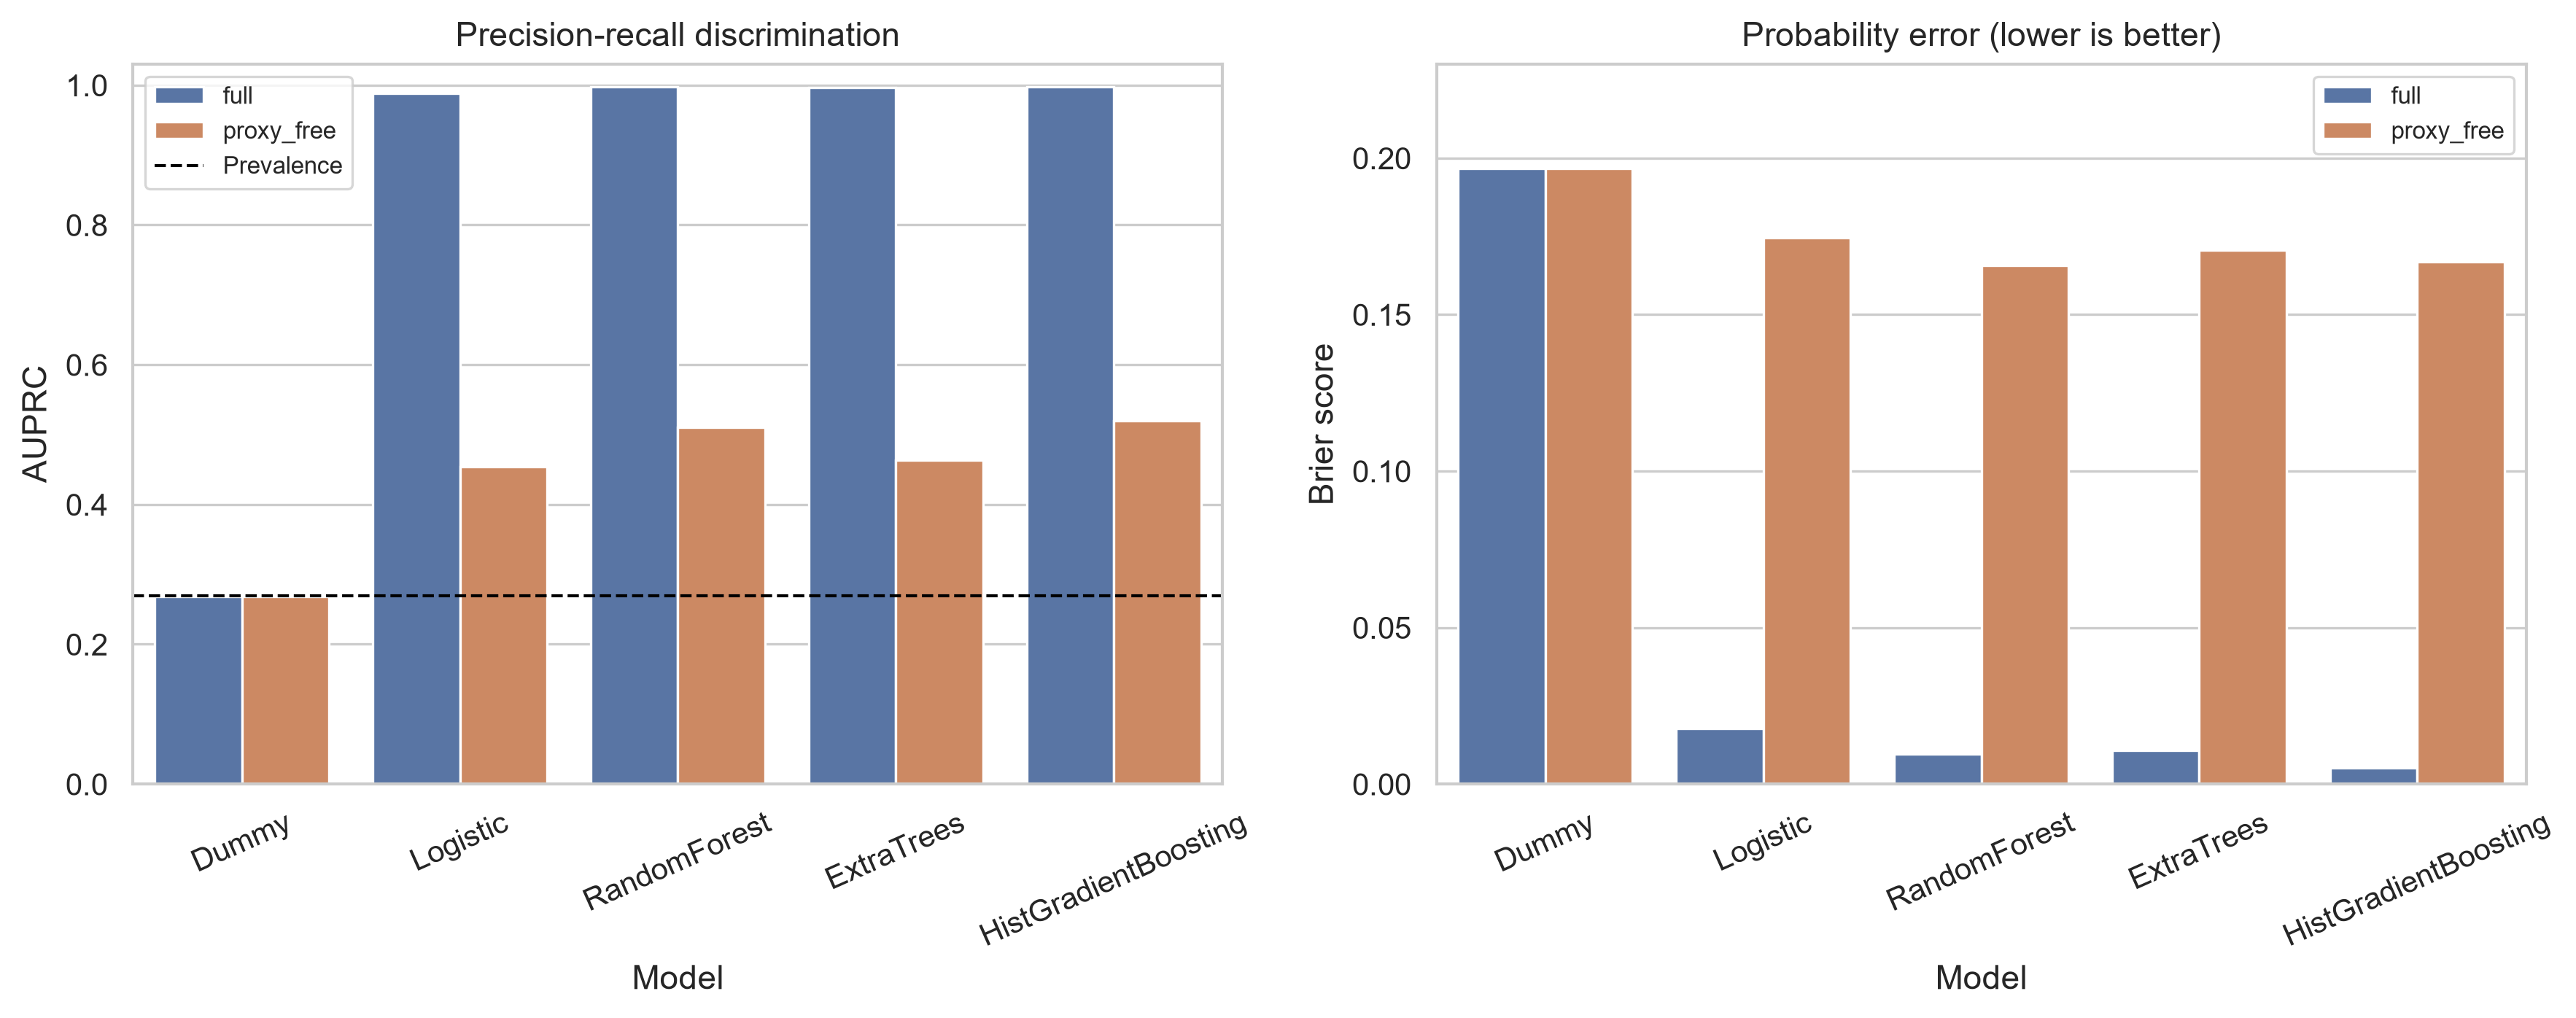
\includegraphics[width=0.92\textwidth]{../artifacts/figures/figure_8_all_model_comparison.png}
\caption{All-model comparison across full and proxy-free feature settings. AUPRC measures ranking under class imbalance; Brier score measures probability error and is lower when better.}
\label{fig:models}
\end{figure*}

Figure~\ref{fig:curves} shows OOF discrimination. The proxy-free model improves substantially over the 0.269 prevalence baseline but has limited sensitivity at a 0.5 threshold. This illustrates why ranking metrics and threshold behavior must be reported together.

\begin{figure}[t]
\centering
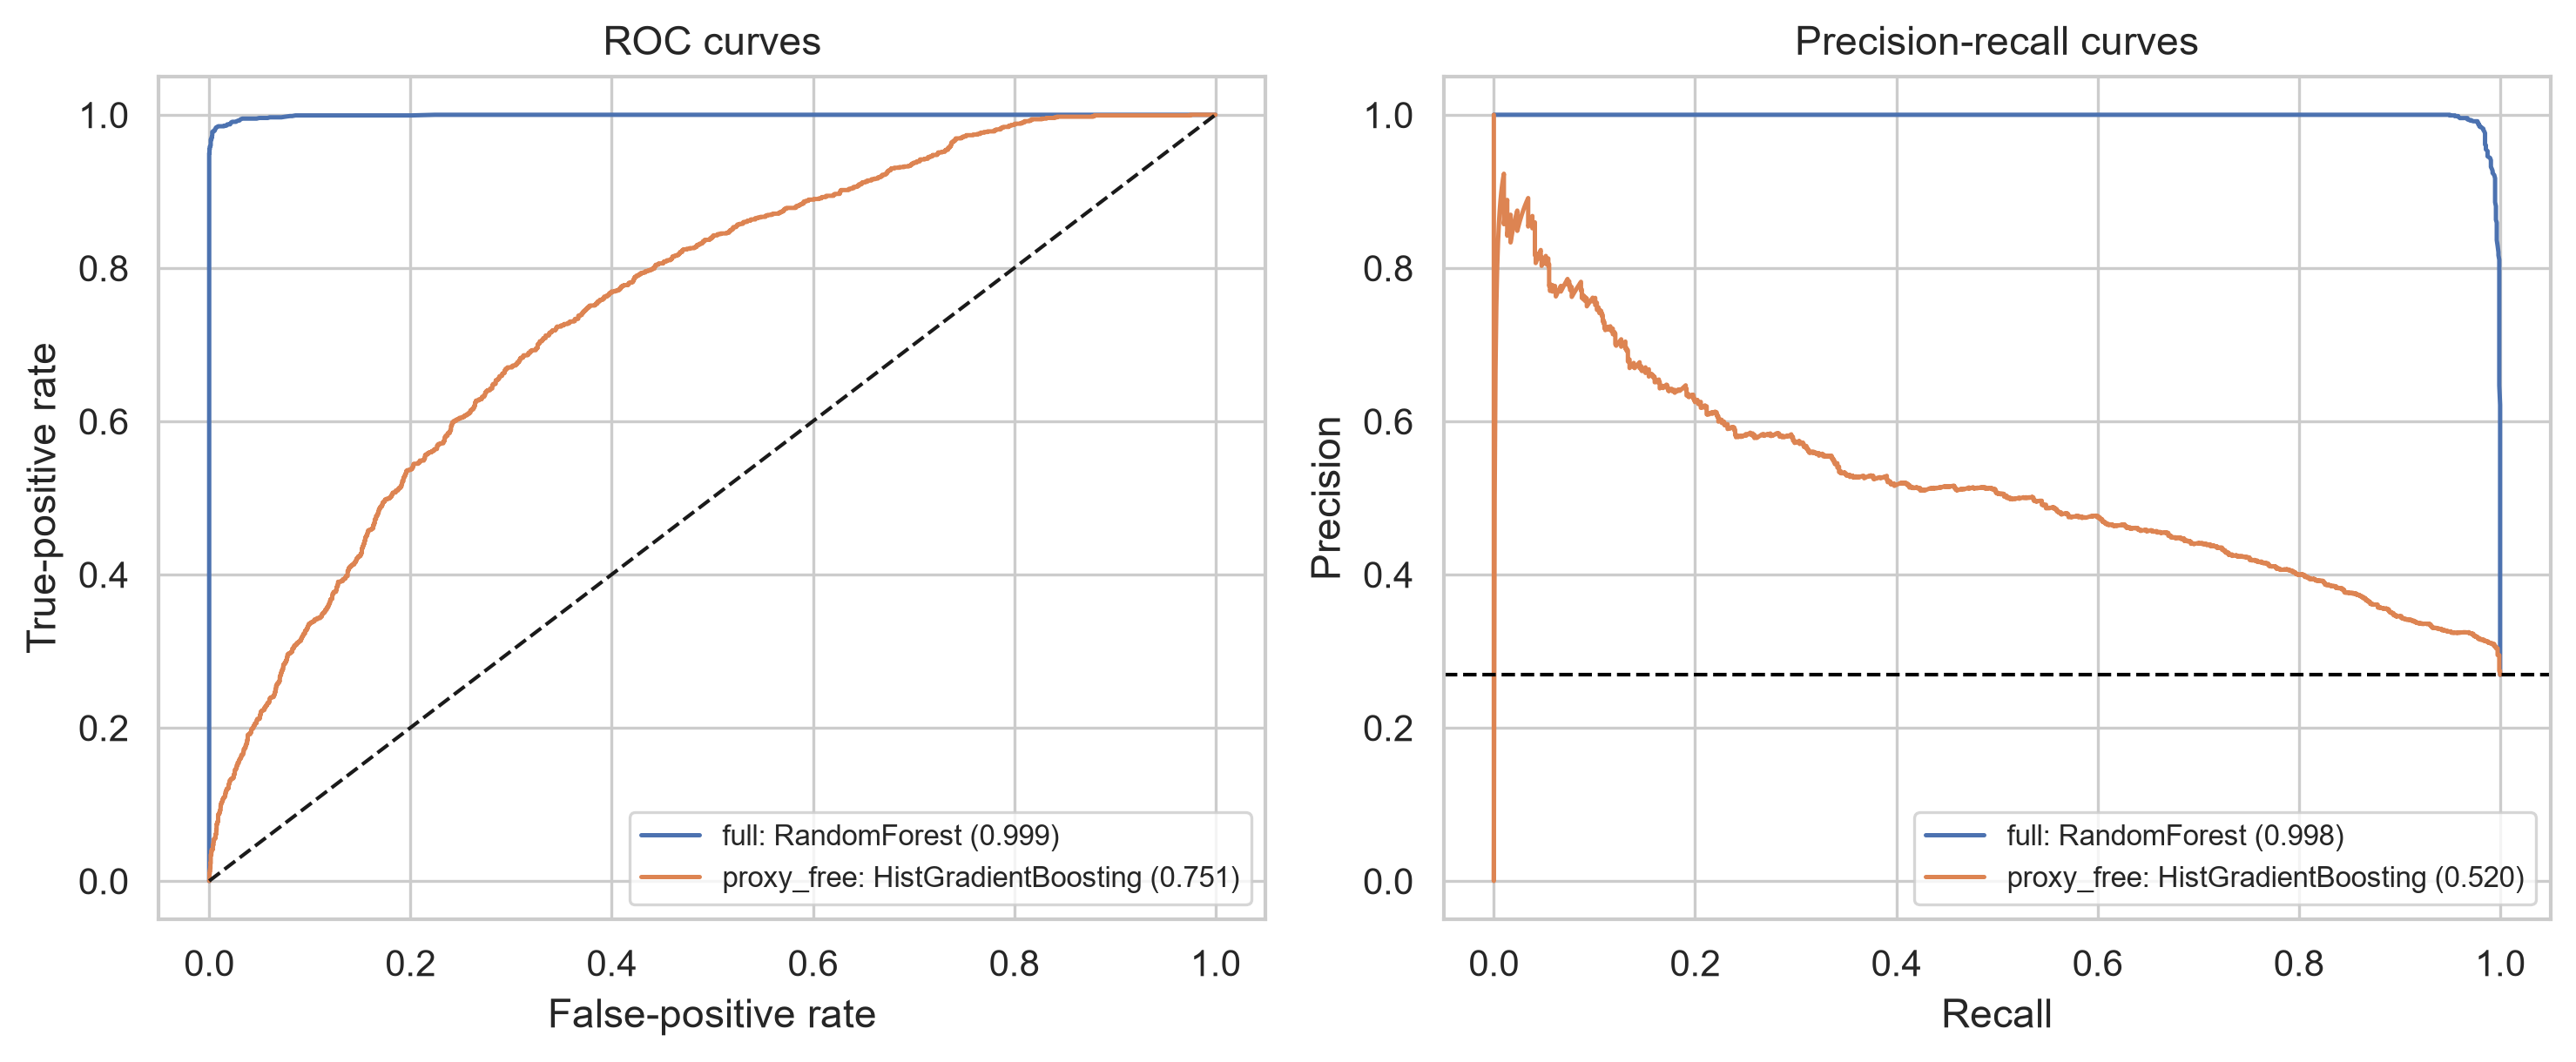
\includegraphics[width=\columnwidth]{../artifacts/figures/figure_3_discrimination_curves.png}
\caption{Out-of-fold ROC and precision--recall curves for selected full and proxy-free models.}
\label{fig:curves}
\end{figure}

The OOF calibration curves in Figure~\ref{fig:calibration} further distinguish discrimination from probability reliability. The full model concentrates predictions close to the empirical extremes, while the proxy-free curve shows larger departures from the identity line. These probabilities would require external recalibration before any threshold-based workflow.

\begin{figure}[t]
\centering
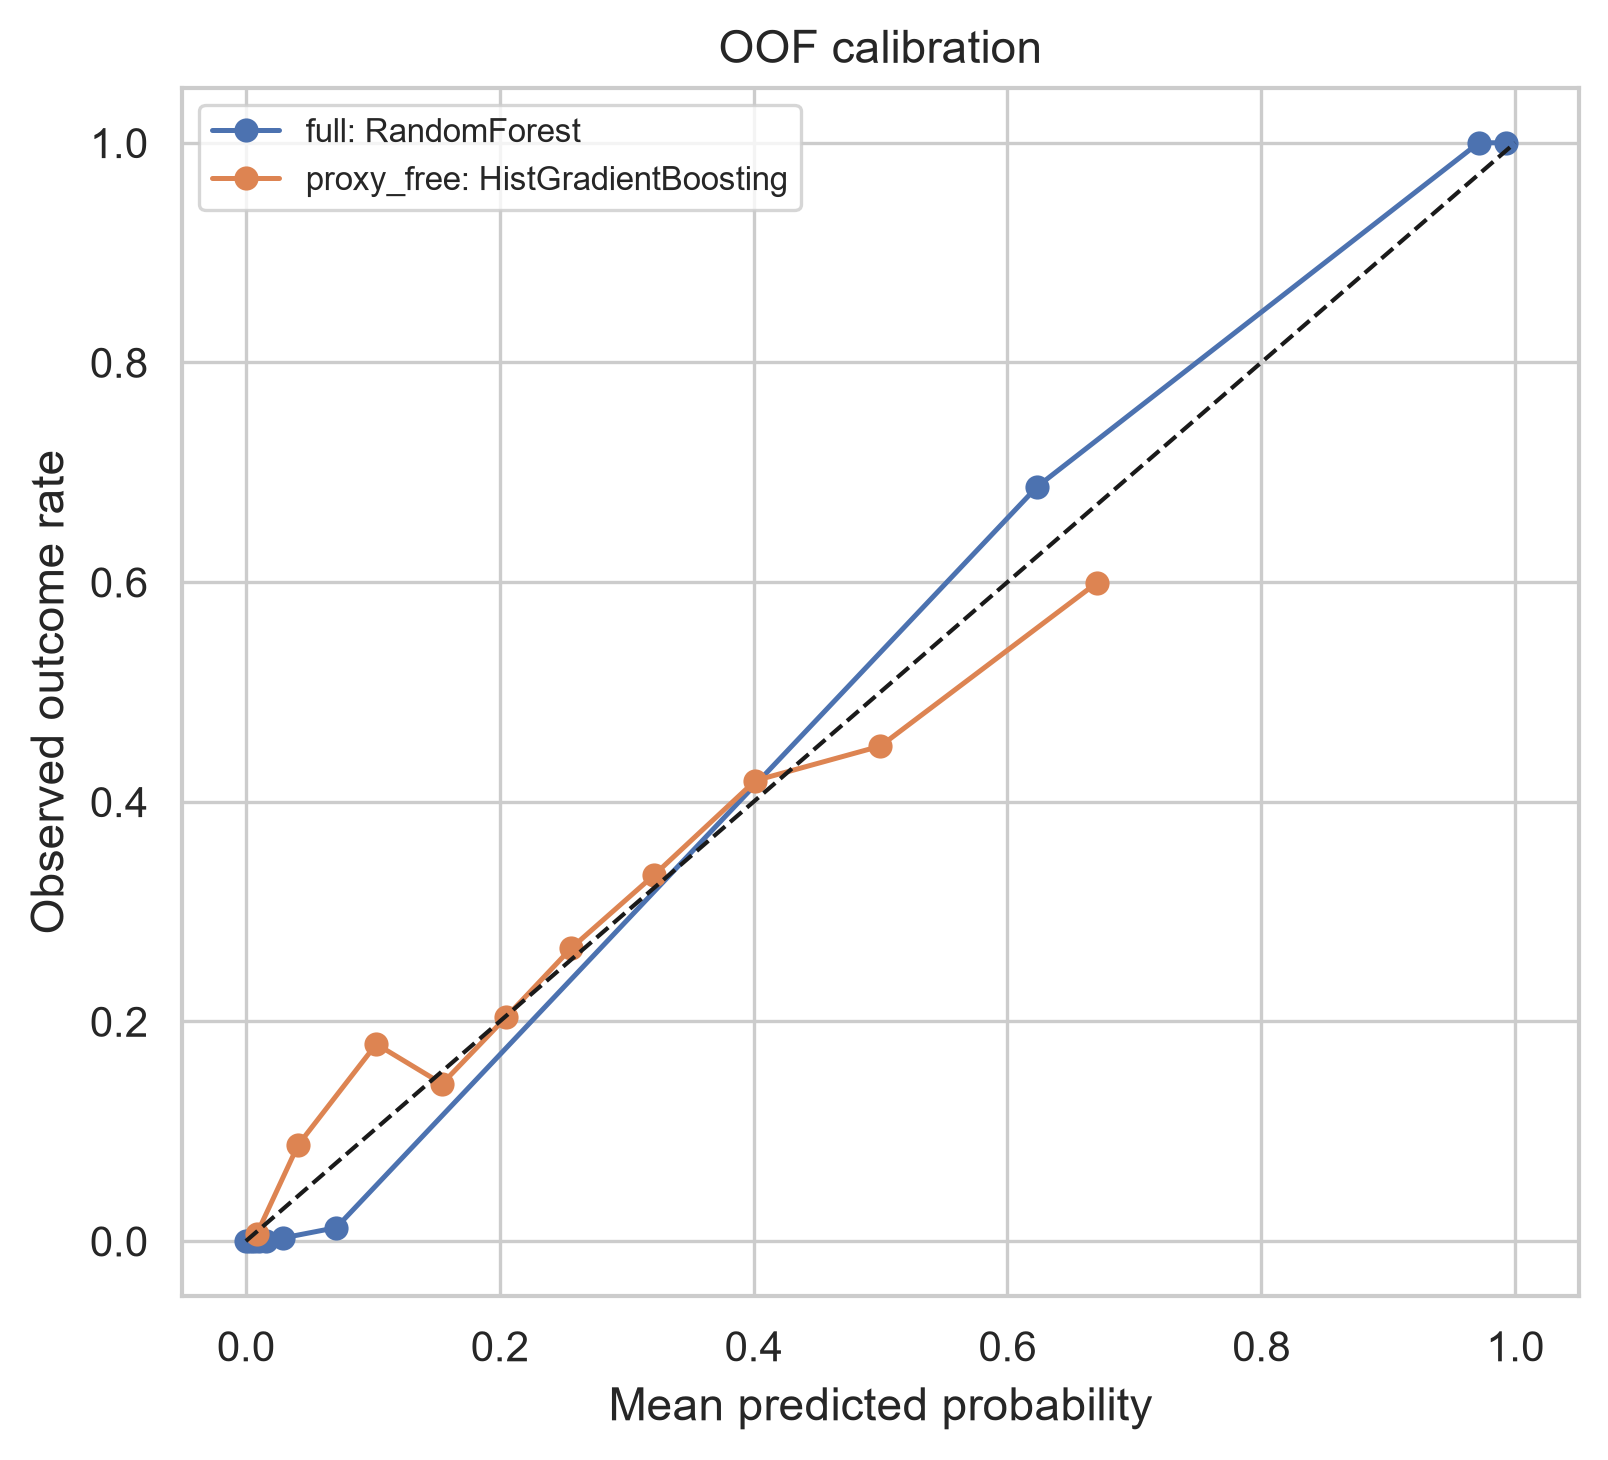
\includegraphics[width=0.88\columnwidth]{../artifacts/figures/figure_4_calibration.png}
\caption{Quantile-binned OOF calibration for selected models.}
\label{fig:calibration}
\end{figure}

\subsection{Geographic-group transportability}
The full model remained near-perfect when each home division was held out (AUPRC 0.998, AUROC 0.999), consistent with the health-condition association persisting across divisions. The proxy-free model declined to AUPRC 0.452, AUROC 0.691, and Brier score 0.184 (Table~\ref{tab:geo}). Proxy-free division-specific AUPRC ranged from 0.393 in Dhaka to 0.551 in Khulna; because prevalence differed, AUPRC should be interpreted together with each division's baseline.

\begin{table}[t]
\centering
\caption{Pooled leave-one-home-division-out performance.}
\label{tab:geo}
\begin{tabular}{lcccc}
\toprule
Setting & AUROC & AUPRC & Brier & F1 \\
\midrule
Full & 0.999 & 0.998 & 0.010 & 0.977 \\
Proxy-free & 0.691 & 0.452 & 0.184 & 0.362 \\
\bottomrule
\end{tabular}
\end{table}

\begin{figure}[t]
\centering
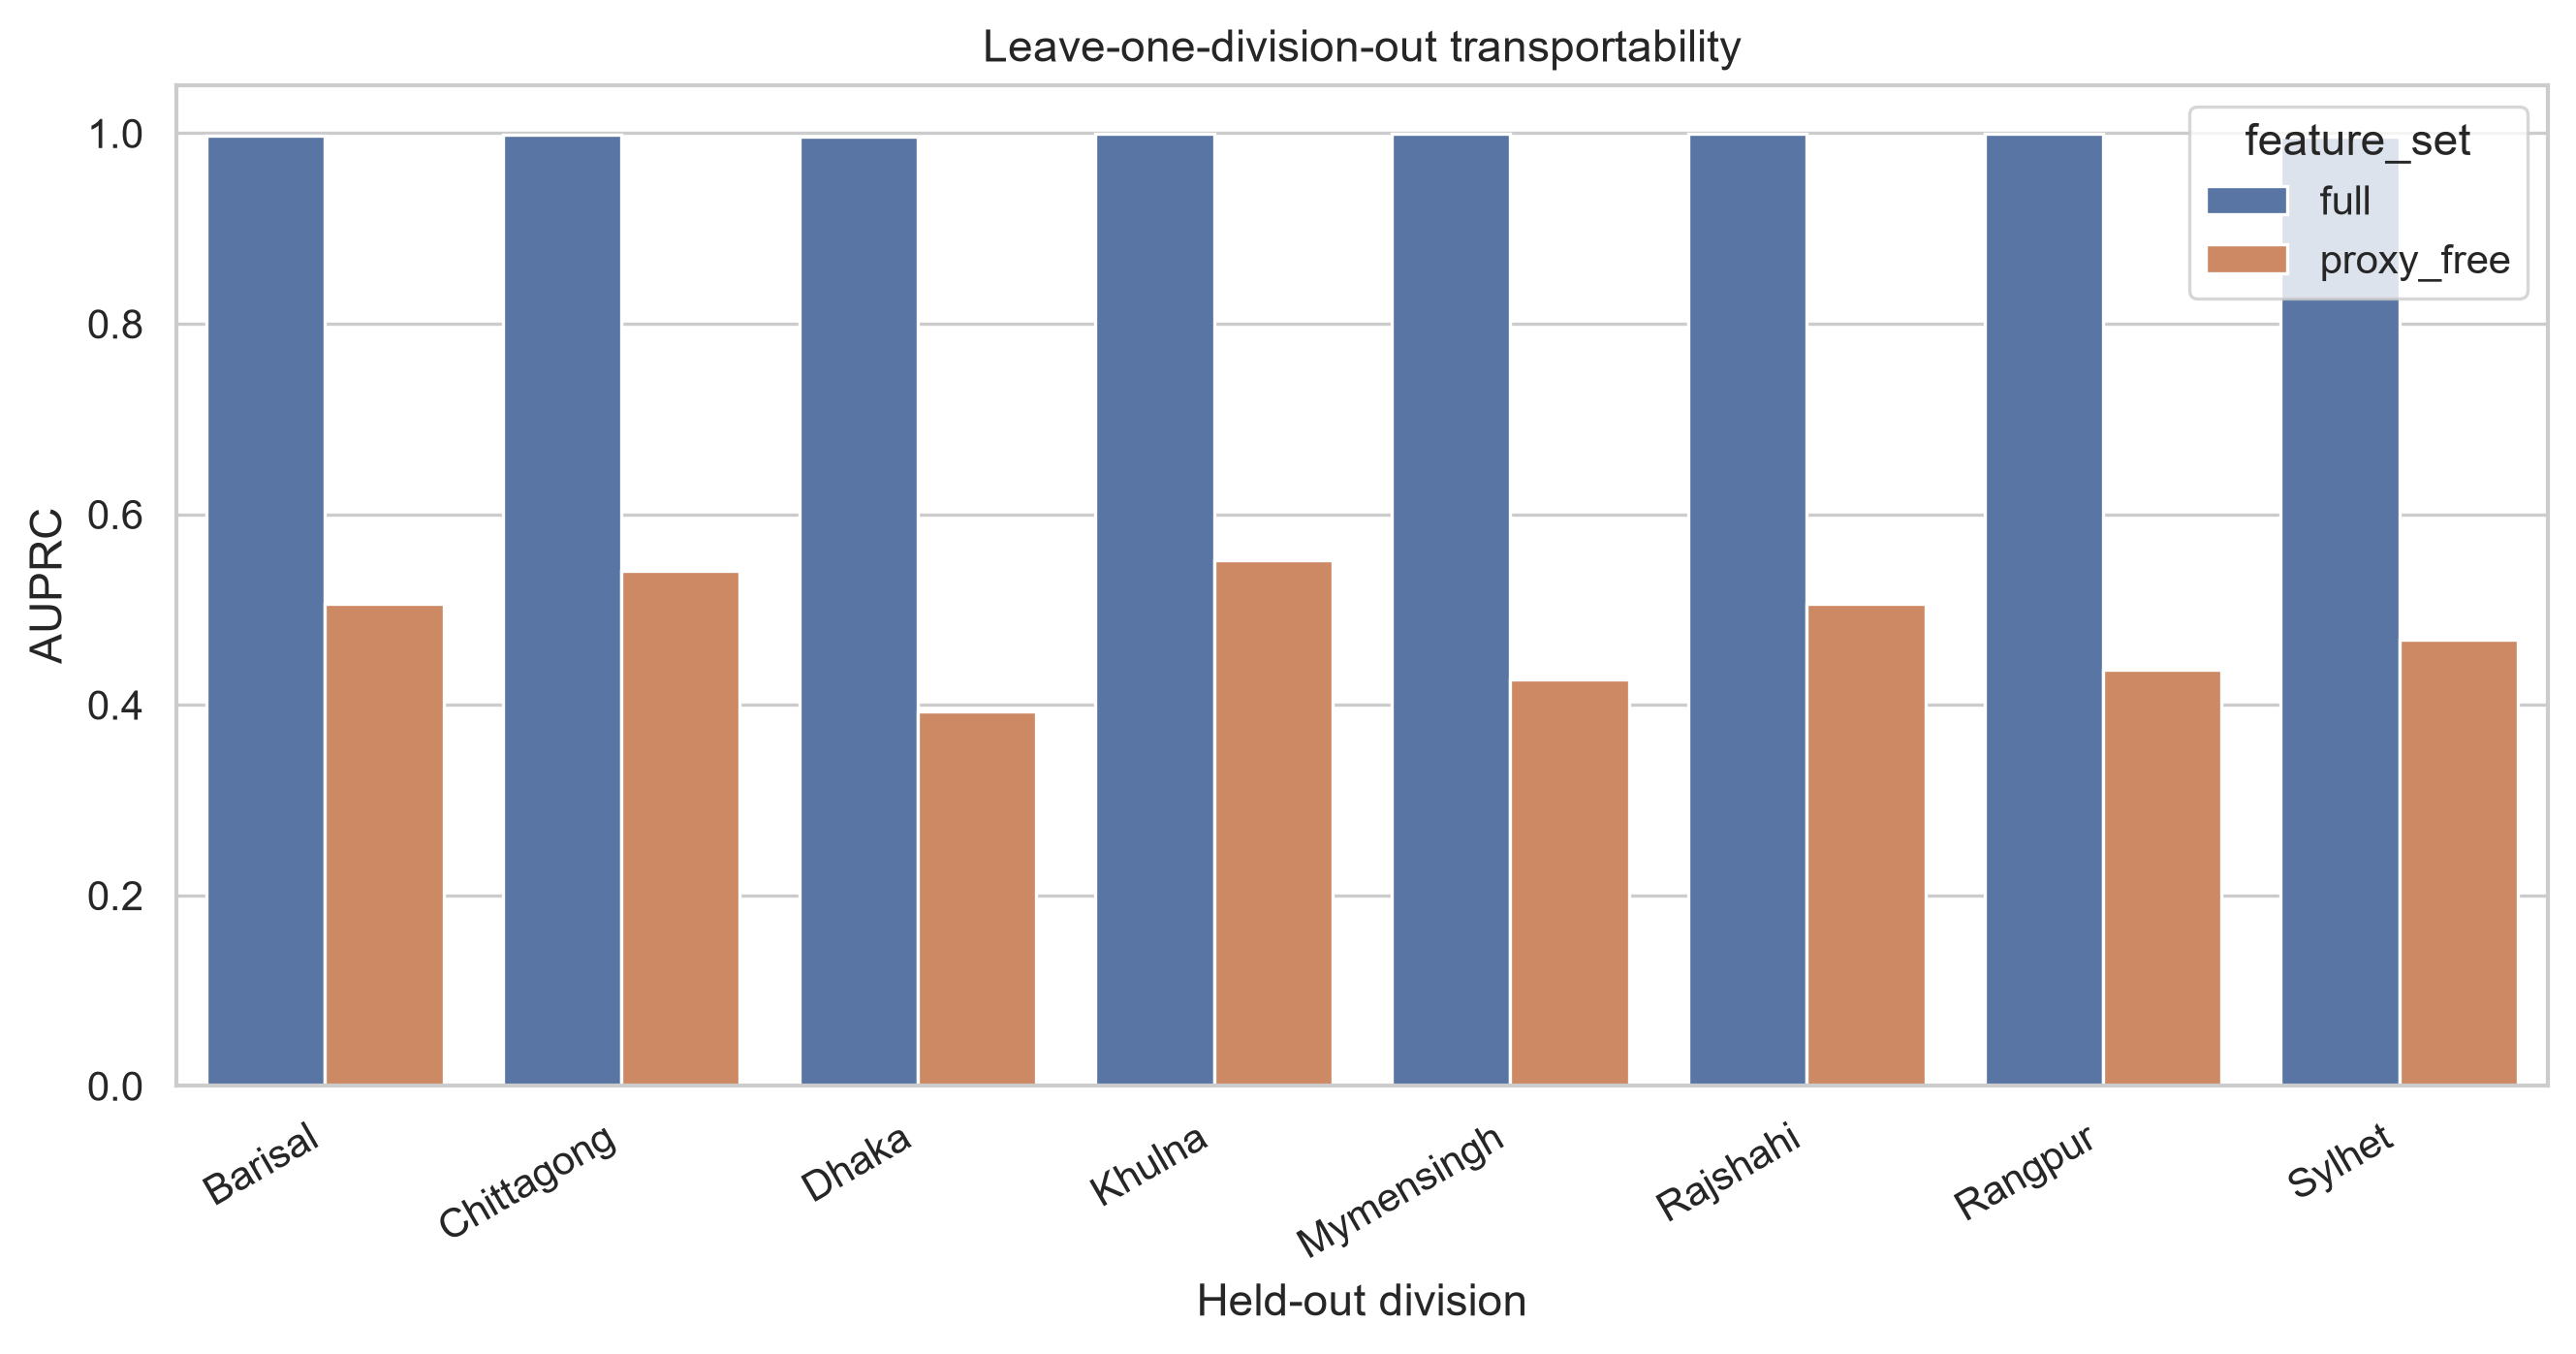
\includegraphics[width=\columnwidth]{../artifacts/figures/figure_5_geographic_transportability.png}
\caption{AUPRC when each home division is held out.}
\label{fig:geo}
\end{figure}

\subsection{Subgroup reliability}
Gender gaps were small for both settings: the proxy-free FNR gap was 0.008 and FPR gap was 0.022. This should not be read as proof of fairness. Larger differences appeared across family background (FNR gap 0.188) and home division (FNR gap 0.284; FPR gap 0.082; Brier gap 0.049) in the proxy-free setting. The full model's corresponding division FNR gap was 0.059. The reduction in aggregate performance therefore coincided with greater geographic heterogeneity.

Figure~\ref{fig:fairness} makes the practical asymmetry visible. In the proxy-free setting, false-negative rates are consistently much larger than false-positive rates at threshold 0.5 and vary materially by division. A high specificity combined with a high FNR is not an acceptable substitute for a clinically selected operating point.

\begin{figure*}[t]
\centering
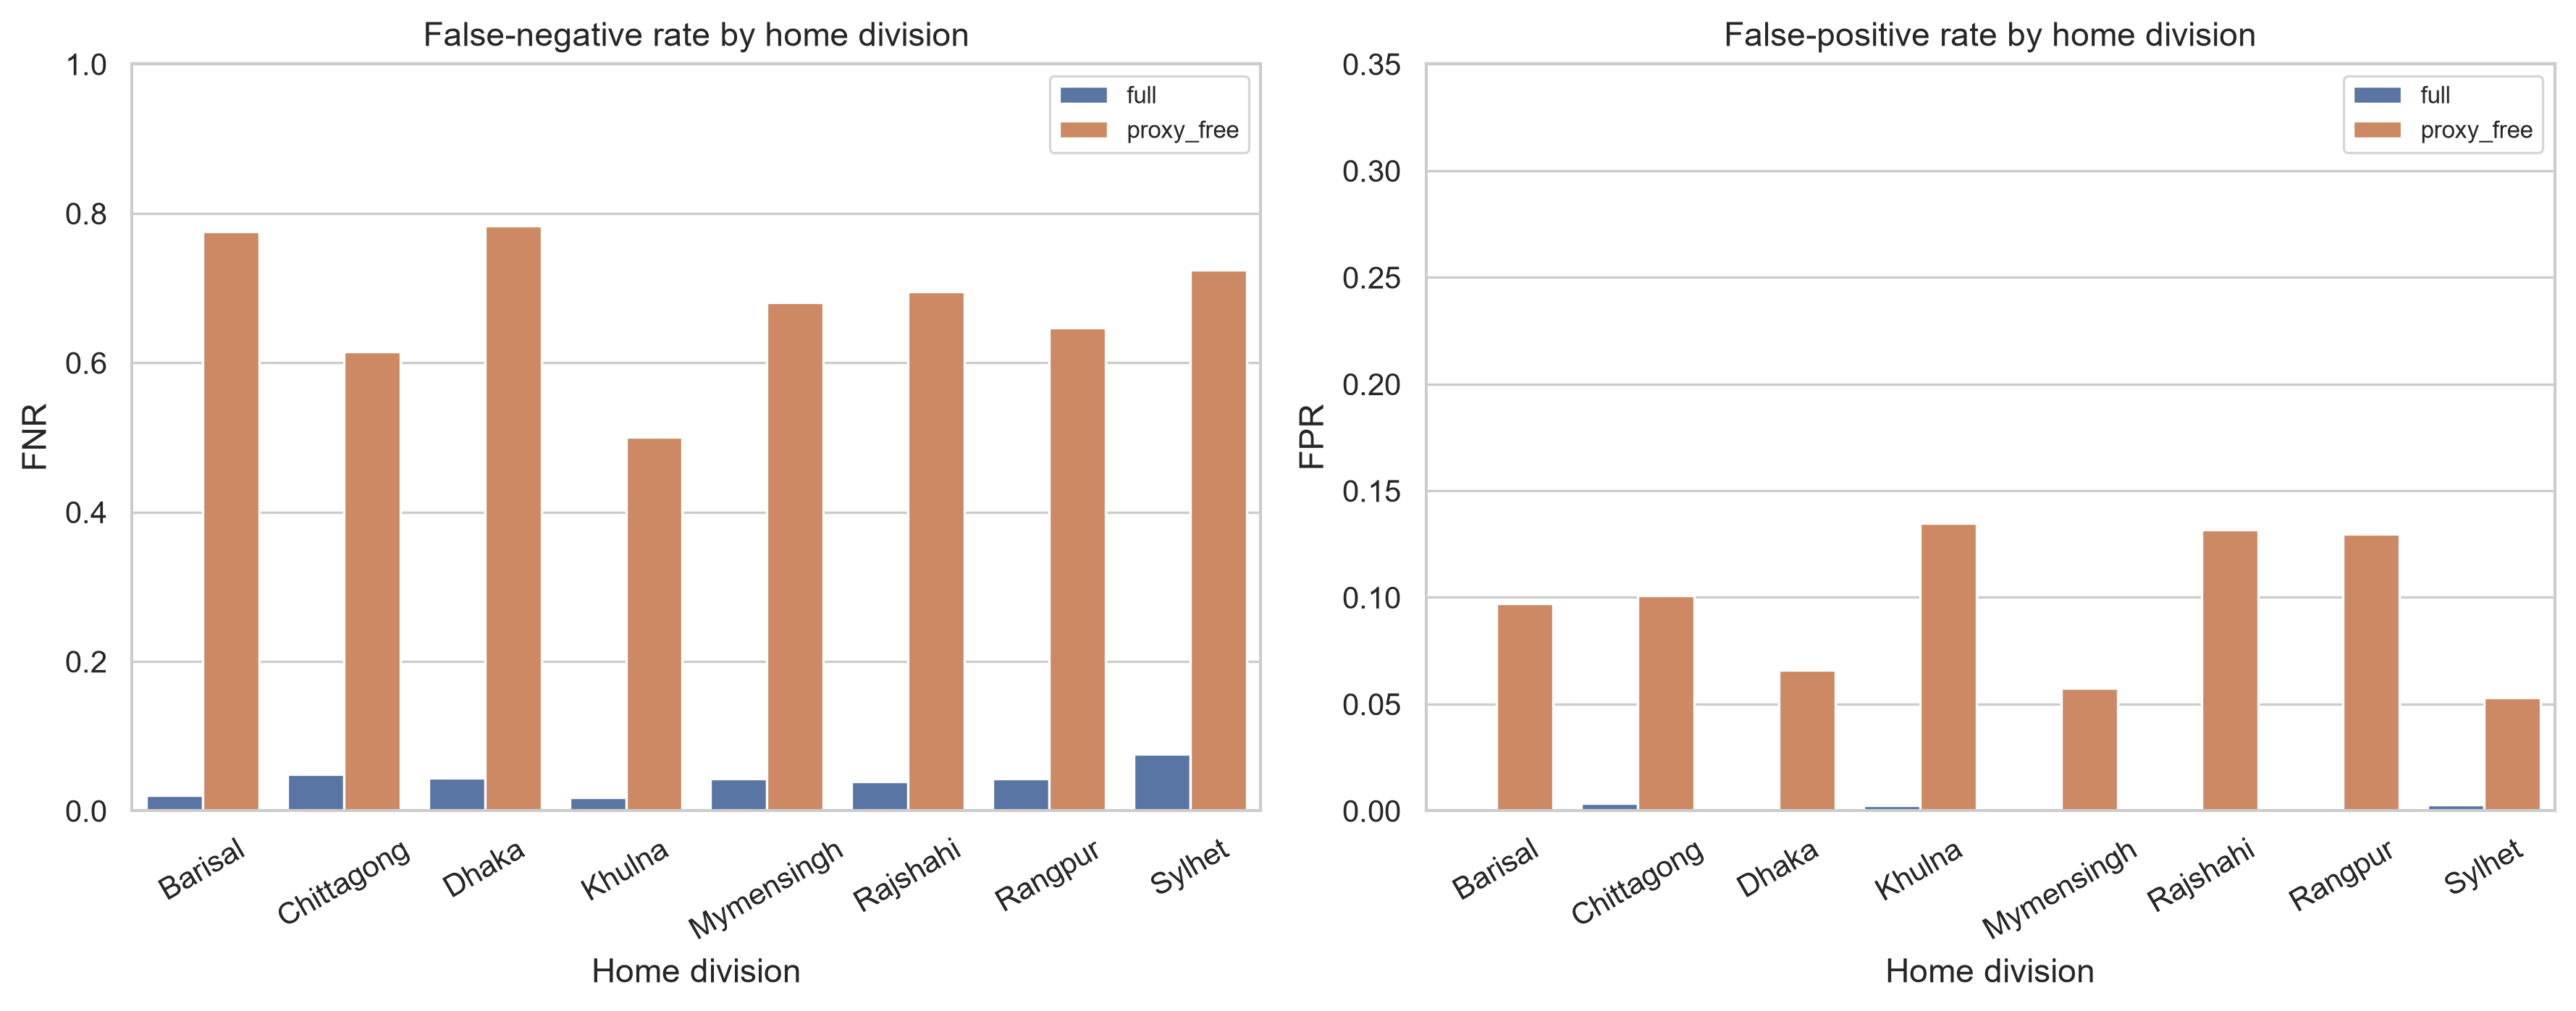
\includegraphics[width=0.92\textwidth]{../artifacts/figures/figure_9_division_error_disparity.png}
\caption{Division-level false-negative and false-positive rates for selected full and proxy-free models at threshold 0.5.}
\label{fig:fairness}
\end{figure*}

\subsection{Uncertainty}
Across five independent 90\% split-conformal runs, mean coverage was 0.903 (range 0.887--0.910), mean set size was 1.391, and 60.9\% of cases received singleton sets. Mean singleton accuracy was 0.841. No empty sets occurred. The conformal procedure achieved its marginal target on average, but roughly two in five cases required a two-label set. This is evidence for explicit uncertainty handling, not a guarantee of clinical safety.

Figure~\ref{fig:conformal} shows run-to-run variability. One split fell below nominal coverage (0.887), as finite-sample marginal validity is probabilistic across random calibration/test draws. Singleton rates varied from 0.560 to 0.657, demonstrating that nominal coverage alone does not describe informativeness.

\begin{figure}[t]
\centering
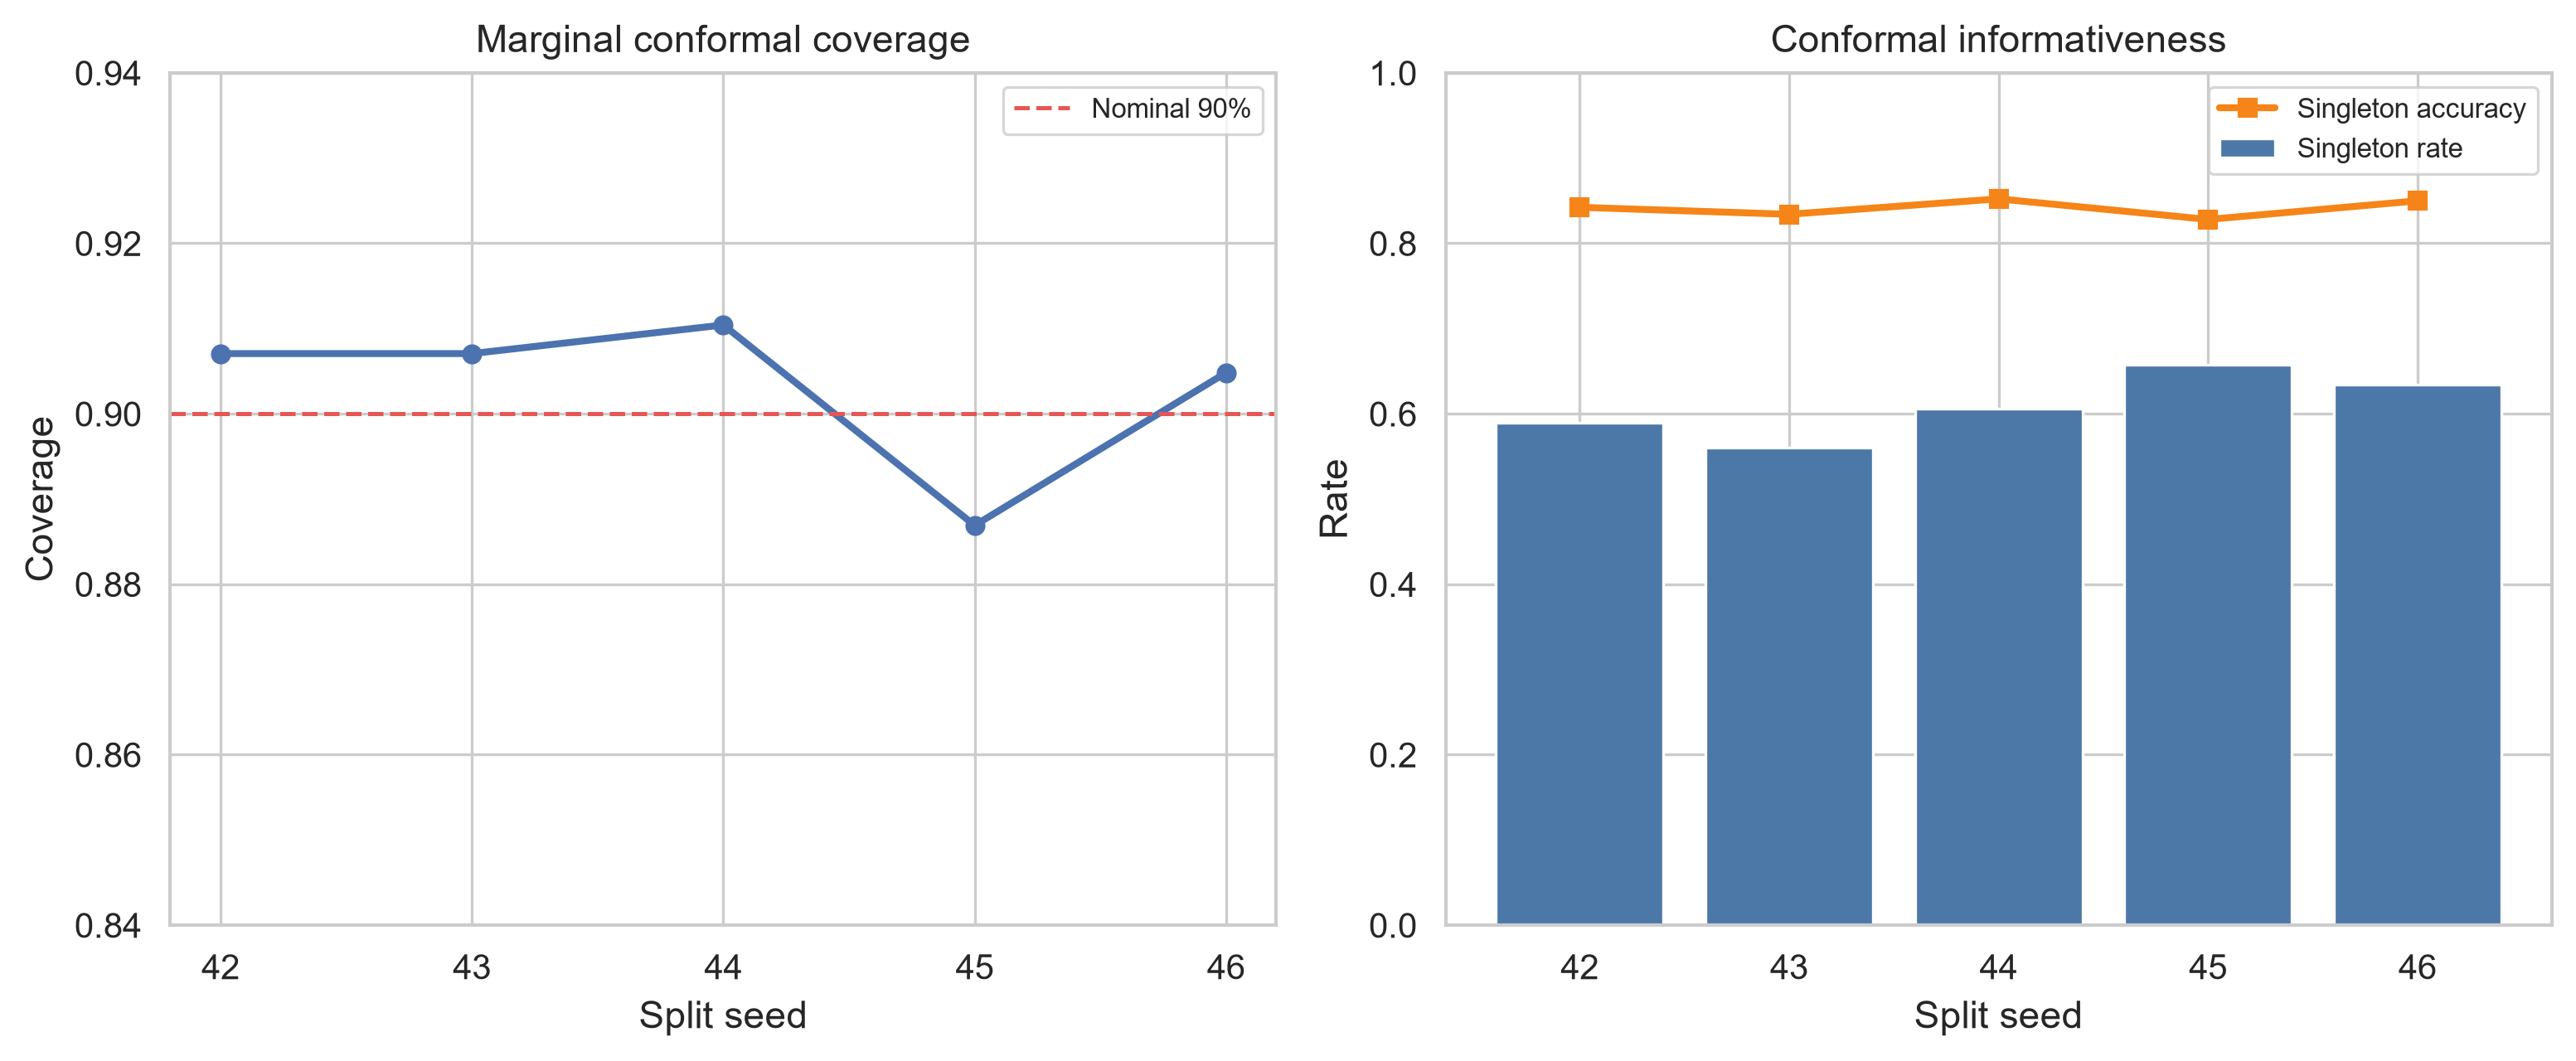
\includegraphics[width=\columnwidth]{../artifacts/figures/figure_10_conformal_reliability.png}
\caption{Repeated split-conformal coverage, singleton rate, and singleton accuracy.}
\label{fig:conformal}
\end{figure}

\section{Discussion}
The central finding is not that Random Forest can obtain near-perfect scores. It is that those scores are highly sensitive to one self-reported variable whose categories almost partition the binary outcome. Without documented questionnaire wording, health condition may be a legitimate concurrent correlate, a component of how respondents understand depression, or an outcome-derived proxy. Each interpretation limits claims of early non-clinical screening.

The proxy-free model retained moderate ranking information internally, but its sensitivity at threshold 0.5 was only 0.312 and performance declined in division-held-out evaluation. This distinction matters operationally. An institution interested in screening would care strongly about missed positive cases, calibration, referral capacity, privacy, and harms of false alerts---not only AUROC.

Our results complement explainable student-depression research \cite{chang2026interpretable,isiwu2026multilevel}: explanations of a high-performing model are insufficient if the model's dominant construct would be unavailable, inappropriate, or tautological at the intended decision time. A feature-exclusion stress test should precede narrative interpretation of feature importance.

Conformal prediction offered a transparent abstention mechanism. Its 90\% marginal coverage came with non-singleton sets for 39.1\% of cases. This trade-off can be appropriate when uncertainty triggers human assessment, but only if referral resources, consent, confidentiality, and response protocols exist. WHO guidance emphasizes autonomy, transparency, accountability, inclusiveness, and safety for AI in health \cite{who2021ethics}; the present evidence does not justify deployment.

\section{Limitations}
First, outcome construction is undocumented beyond a binary label; the absence of a validated scale prevents diagnostic interpretation. Second, the cross-sectional design cannot establish temporal prediction or causality. Third, recruitment, response rate, collection period, non-response, and sampling frame are not fully reported in the public data card, limiting selection-bias assessment. Fourth, home division is not an independent collection site, so leave-one-division-out evaluation is weaker than external validation at a new university or time period. Fifth, the dataset includes only binary gender labels and cannot assess broader gender diversity. Sixth, subgroup estimates were not accompanied by multiplicity-adjusted hypothesis tests; they are audits rather than inferential fairness claims. Seventh, conformal validity assumes exchangeability and is not subgroup-conditional. Finally, no prospective workflow, clinician comparison, decision-curve analysis, or impact evaluation was performed.

\section{Conclusion}
Near-perfect internal performance on this public student-depression dataset is not robust evidence of deployable screening. A single potential outcome proxy explains much of the apparent predictability; excluding it substantially reduces AUPRC and reveals geographic-group heterogeneity and frequent uncertainty. Student mental-health prediction studies should document the outcome instrument and prediction time, perform proxy-exclusion sensitivity analyses, evaluate calibration and subgroup errors, and seek external validation before clinical or institutional claims. Our executed notebook and complete OOF predictions make this audit reproducible.

\section*{Data and Code Availability}
The source dataset is public under CC BY 4.0 \cite{haque2026dataset}. The accompanying repository contains the executed notebook, analysis module, hyperparameter records, OOF predictions, figures, and CSV tables. No model or output should be used to diagnose or rank students.

\section*{Ethics Statement}
This study analyzes an existing de-identified public dataset and does not contact participants or make individual decisions. Any future primary data collection or deployment requires institutional ethics review, informed consent, privacy safeguards, and a human-led support pathway.

\bibliographystyle{IEEEtran}
\bibliography{references}
\end{document}
